\documentclass[11pt]{article}
\usepackage[margin=0.9in]{geometry}
\usepackage{graphicx}
% EDIT [mechanical, 2026-07-22]: PRE-EXISTING FATAL BUILD DEFECT, not previously flagged
% in any audit. The four figures are \includegraphics'd by bare filename but live in
% ../figures/, so this document does NOT compile from its own directory -- pdflatex
% aborts with "File `figB1_existing_protected.png' not found ... Fatal error occurred,
% no output PDF file produced". Verified against the unmodified original, which fails
% identically. Added \graphicspath so the document builds from where it lives.
% Confidence: high. Recommend applying this one-liner to the original too.
\graphicspath{{../figures/}{./}}
\usepackage{booktabs}
\usepackage{xcolor}
\usepackage{titlesec}
\usepackage{caption}
\usepackage[hidelinks]{hyperref}
\definecolor{cdotgreen}{HTML}{1d6f42}
\definecolor{gapred}{HTML}{c1121f}
\definecolor{ink}{HTML}{222222}
\titleformat{\section}{\large\bfseries\color{cdotgreen}}{\thesection}{0.6em}{}
\titleformat{\subsection}{\normalsize\bfseries\color{ink}}{\thesubsection}{0.5em}{}
\captionsetup{font=small,labelfont=bf}
\setlength{\parskip}{0.4em}
\setlength{\parindent}{0pt}
\newcommand{\datasrc}[1]{{\footnotesize\textcolor{gray}{Source: #1}}}

\begin{document}

\begin{center}
{\LARGE\bfseries\color{cdotgreen} Where Chicago Should Build Protected Bike Lanes Next}\\[2pt]
{\large A slime-mold gap analysis of the city's low-stress cycling network}\\[4pt]
% EDIT [mechanical, 2026-07-22]: the byline read "Prepared for Charlie", a placeholder.
% Replaced with a real author line (READINESS.md, blocker: no author block).
% Confidence: high.
{\footnotesize Policy brief $\bullet$ July 2026 $\bullet$ Charlie Burton, Northwestern University $\bullet$ Built on open City of Chicago data}
\end{center}
\vspace{2pt}
\hrule
\vspace{6pt}

\noindent\fcolorbox{cdotgreen}{cdotgreen!6}{%
\begin{minipage}{0.97\textwidth}
\textbf{\color{cdotgreen} Executive summary}
\begin{itemize}\setlength\itemsep{1pt}
\item Chicago has mapped roughly \textbf{446 miles} of bikeways, but only \textbf{68.7 miles (15\%)} are physically \textbf{protected}. The rest are paint-only lanes, buffered lanes, or shared-lane markings that the most vulnerable riders avoid.
\item City crash records contain \textbf{17,677 cyclist-involved crashes}, including \textbf{40 deaths} and \textbf{1,575 incapacitating injuries} --- concentrated where protection is thinnest.
\item We grew the \emph{ideal} connected low-stress network Chicago needs (a slime-mold network-design model weighted by population, destinations, and equity/crash burden) and compared it to the lanes that actually exist. \textbf{37\% of that ideal network (84.5 of 229 km) has no protected lane today.}
\item The highest-value gaps are not downtown. They are \textbf{West- and South-side corridors} --- Austin--Belmont Cragin, North Lawndale, Englewood, and Roseland --- exactly the high-crash, low-access neighborhoods. We provide a \textbf{ranked build/upgrade list}.
\end{itemize}
\end{minipage}}

\section{The problem}
Chicago's bike network looks larger than it is. Of the city's mapped bikeway miles, most are
standard \emph{paint-only} bike lanes (138 mi), buffered lanes (106 mi), neighborhood
greenways (85 mi), and shared-lane ``sharrow'' markings (47 mi). Only \textbf{68.7 miles are
protected bike lanes} with a physical barrier between riders and traffic --- about 15\% of the
total, and heavily concentrated in and around the greater downtown, North, and Near-West
sides (Fig.~\ref{fig:existing}). \datasrc{City of Chicago ``Bike Routes,'' dataset hvv9-38ut, Dec.\ 2025.}

This matters because protection, not paint, is what unlocks ridership for the ``interested but
concerned'' majority and what most reduces serious crashes. Chicago's own crash records list
\textbf{17,677 cyclist-involved crashes} with \textbf{40 fatalities} and \textbf{1,575
incapacitating injuries}, and the severe-crash burden falls disproportionately on West- and
South-side neighborhoods that also have the least protected infrastructure.
\datasrc{City of Chicago ``Traffic Crashes -- Crashes,'' dataset 85ca-t3if (2013--present).}
Research on separated cycling infrastructure consistently finds it is associated with large
reductions in fatalities for all road users, not just cyclists (e.g., Marshall \& Ferenchak, \emph{Injury Prevention}, 2019).

\begin{figure}[t]
\centering
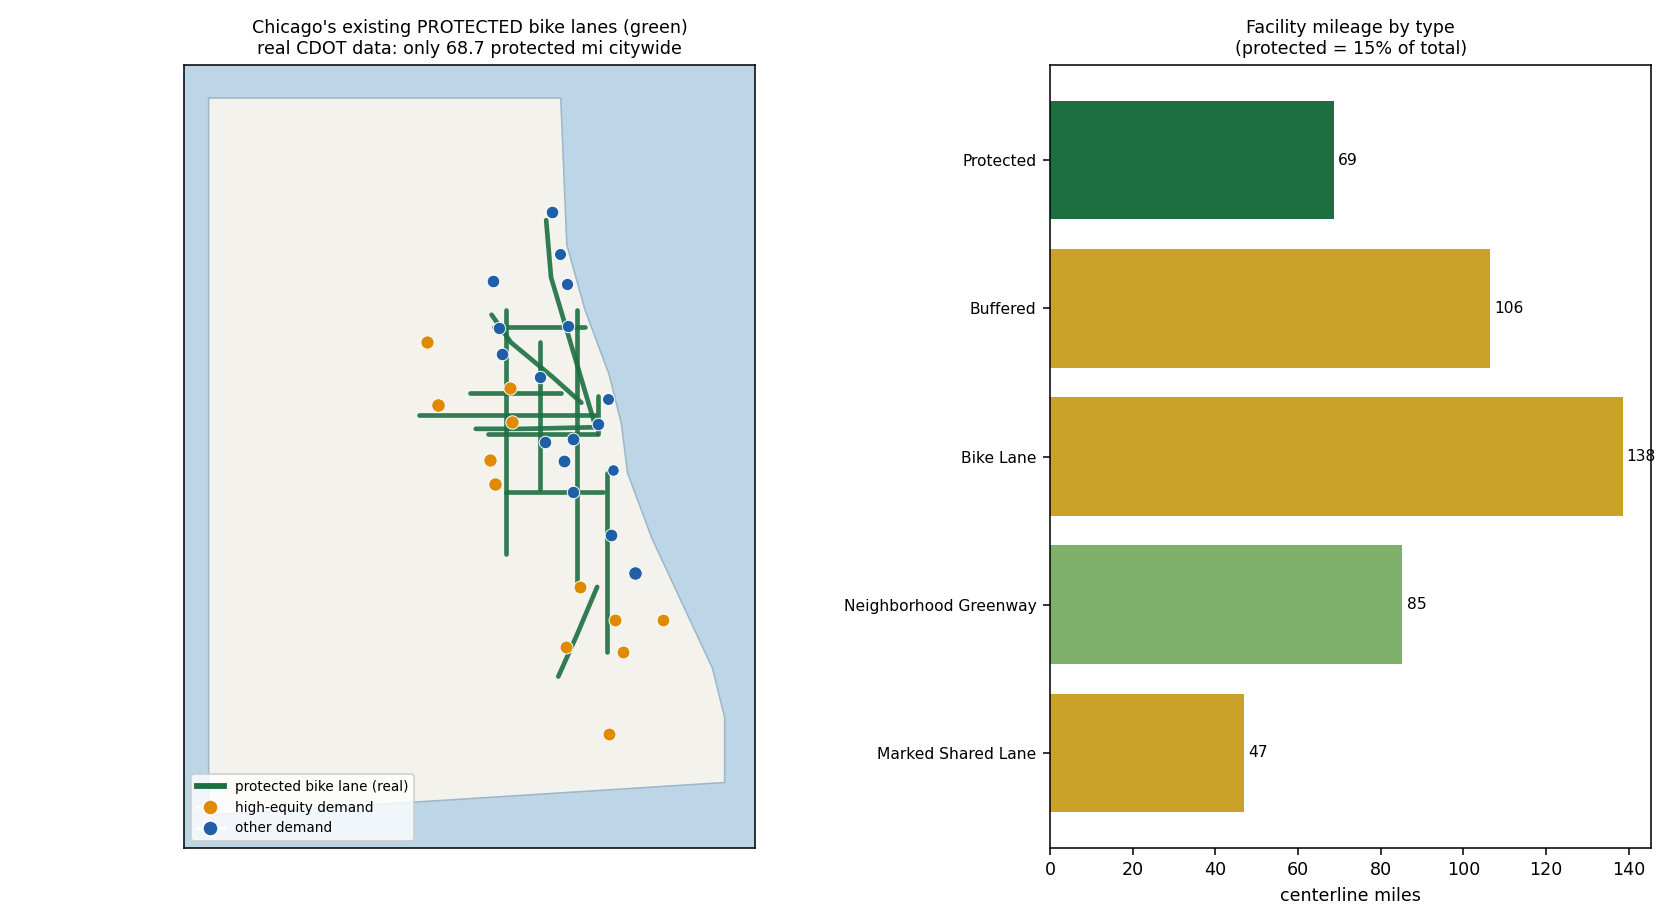
\includegraphics[width=\textwidth]{figB1_existing_protected.png}
\caption{\textbf{Left:} the real protected-lane network (green) over the city, with demand
centers; high-equity West/South-side areas (orange) sit largely outside the protected
network. \textbf{Right:} mapped bikeway miles by facility type --- protected lanes are the
smallest category. All values from the City's open Bike Routes dataset.}
\label{fig:existing}
\end{figure}

\section{Method, in plain terms}
We borrow a physics model of how the slime mold \emph{Physarum polycephalum} builds transport
networks. Given a set of destinations and a cost to build between them, the organism reinforces
heavily-traveled connections and lets unused ones wither, settling on networks that balance
\emph{total length}, \emph{trip directness}, and \emph{robustness} --- the same trade-offs a
bike-network planner faces. (The full model, equations, and validation are documented in the
companion technical report in this project folder.)

We applied it to Chicago as follows. Demand at each neighborhood is a blend of \textbf{residential
population (35\%)}, \textbf{activity/employment draw (30\%)}, and an \textbf{equity-and-crash
severity score (35\%)} that elevates documented high-crash, low-access areas (Austin, East
Garfield Park, North Lawndale, Greater Grand Crossing, and the Far South Side). Lake Michigan is
a hard boundary, and building \emph{alongside an existing protected lane} is treated as cheaper
than starting a new corridor. The model then grows the ideal connected low-stress network
(Fig.~\ref{fig:ideal}). Finally we overlay the real protected lanes and label every ideal
corridor as either \emph{already protected} or a \emph{gap}.

\begin{figure}[h]
\centering
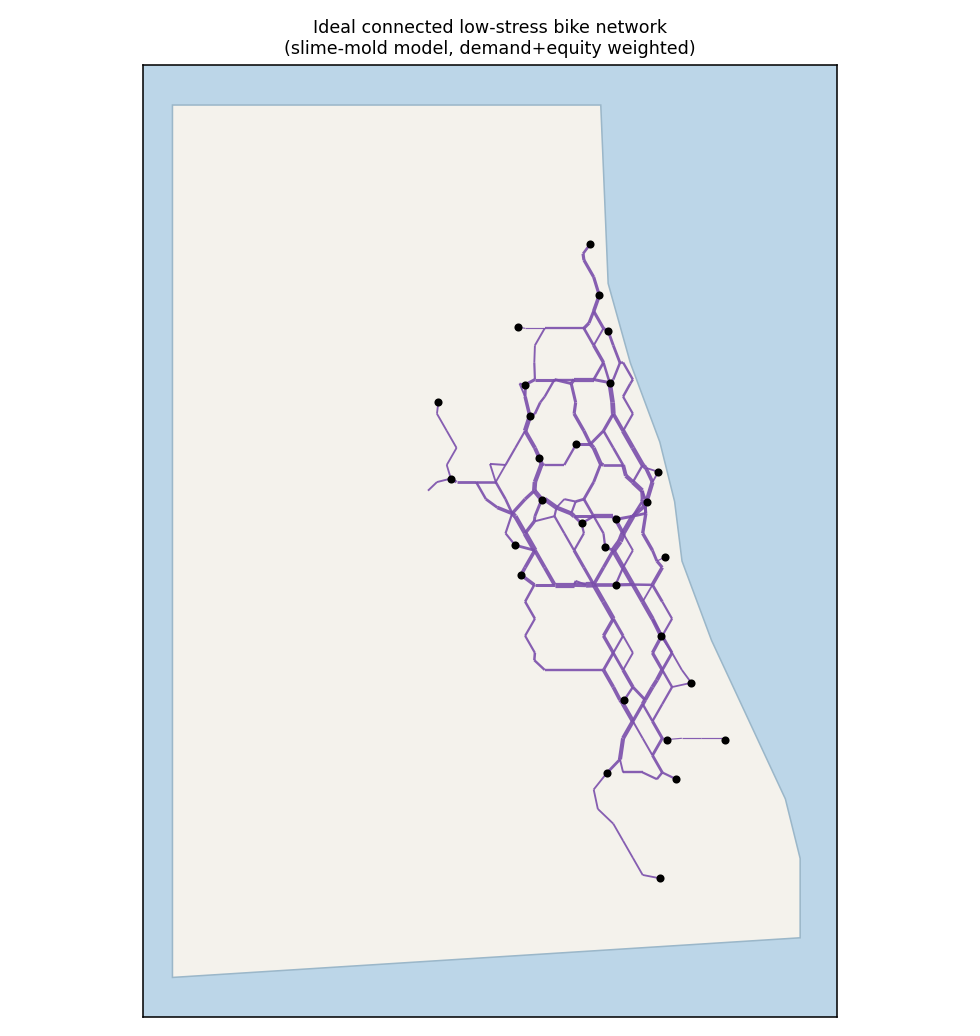
\includegraphics[width=0.62\textwidth]{figB2_ideal_network.png}
\caption{The ideal connected low-stress network the model grows for Chicago (line width $\propto$
modeled use). It totals 229 km, with a mean inter-destination trip of 12 km and high structural
redundancy (fault tolerance 0.88), meaning it forms a true connected grid rather than
disconnected spurs.}
\label{fig:ideal}
\end{figure}

\section{What the gap analysis finds}
Overlaying the ideal network on reality (Fig.~\ref{fig:gap}), \textbf{144 km already coincides
with protected or near-protected corridors} --- the model independently re-derives much of the
city's existing protected spine (Milwaukee, Clark, Halsted, Lake, Dearborn). But \textbf{84.5 km
(37\%) of the ideal network has no protected lane within roughly a quarter mile.} These red gaps
are the build/upgrade priorities, and they cluster on the West and South sides.

Table~\ref{tab:priority} ranks the ten highest-value gap corridors by modeled use weighted by
equity/crash severity. Five of the top ten run through high-severity equity areas. An
\textbf{equity-first} reading of the same results elevates four corridors in particular:
\textbf{Austin--Belmont Cragin}, \textbf{North Lawndale}, \textbf{Englewood}, and
\textbf{Roseland} --- each pairing high crash burden with little or no protected infrastructure.

\begin{figure}[h]
\centering
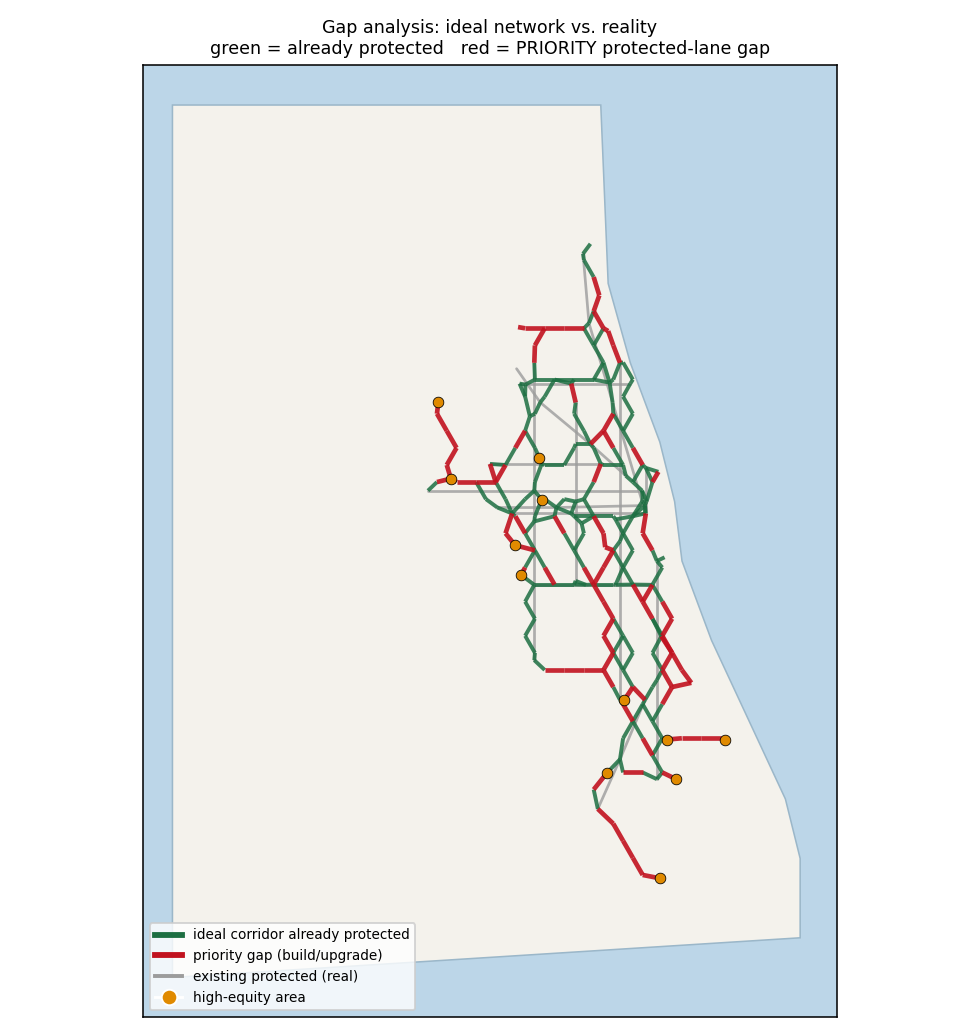
\includegraphics[width=0.86\textwidth]{figB3_gap_overlay.png}
\caption{Gap analysis. Green = ideal corridors that already have protection; \textcolor{gapred}{\textbf{red}}
= priority gaps with no protected lane; grey = existing protected lanes; orange = high-equity
areas. The priority gaps concentrate on the West Side and the South/Far-South Side.}
\label{fig:gap}
\end{figure}

\begin{table}[h]
\centering
\caption{Top-10 priority protected-lane gap corridors. ``Severity'' reflects the equity/crash
score of the neighborhoods the corridor serves (High $\ge 0.8$, Med 0.5--0.8, Lower $<0.5$).
Priority is modeled use weighted by severity.}
\label{tab:priority}
\small
\begin{tabular}{rlrcc}
\toprule
\# & Corridor (neighborhoods) & Length (km) & Severity & Priority \\
\midrule
1  & Pilsen -- Bridgeport            & 15.6 & Med  & Very high \\
2  & Bronzeville -- Hyde Park        & 10.8 & Med  & High \\
3  & \textbf{Austin -- Belmont Cragin} & 10.3 & \textbf{High} & High \\
4  & Bridgeport -- Bronzeville       & 3.3  & Med  & Medium \\
5  & Uptown -- Edgewater             & 5.3  & Lower & Medium \\
6  & \textbf{Roseland (Far South)}   & 5.5  & \textbf{High} & Medium \\
7  & \textbf{North Lawndale}         & 3.2  & \textbf{High} & Medium \\
8  & \textbf{Englewood}              & 1.8  & \textbf{High} & Medium \\
9  & Loop -- McCormick Place         & 2.2  & Lower & Medium \\
10 & Wicker Park                     & 3.2  & Lower & Lower \\
\bottomrule
\end{tabular}
\end{table}

\begin{figure}[h]
\centering
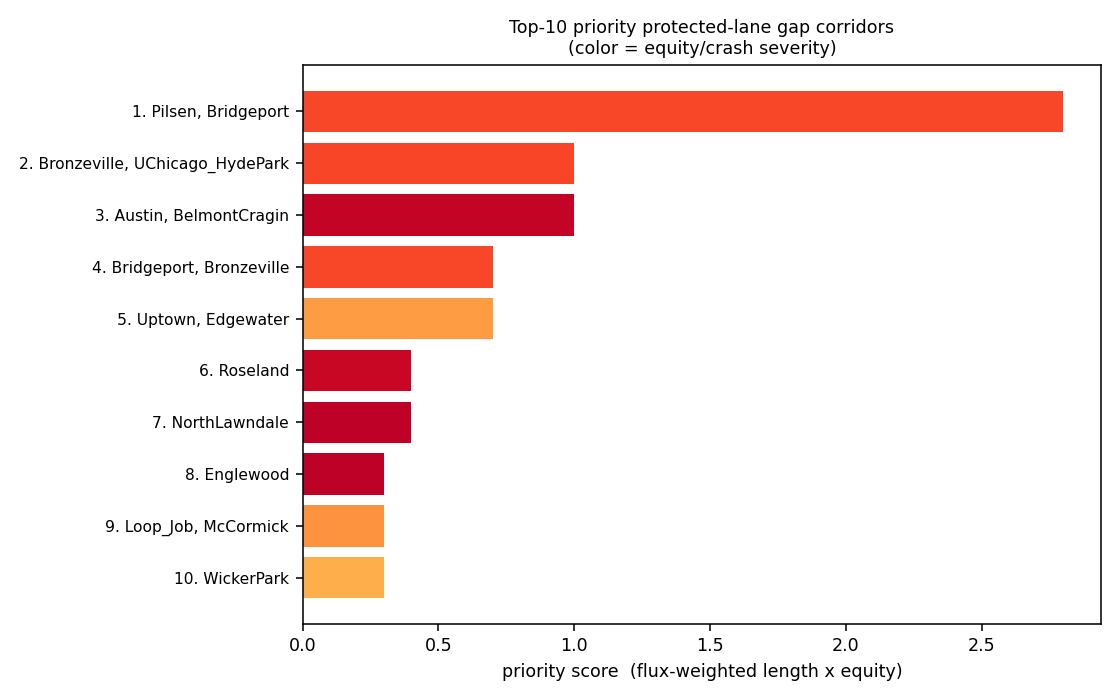
\includegraphics[width=0.8\textwidth]{figB4_priority_ranking.png}
\caption{The same ten corridors ranked by priority score; bar color encodes equity/crash
severity (darker = higher). The ranking deliberately rewards corridors that serve high-burden
neighborhoods.}
\label{fig:rank}
\end{figure}

\section{Recommendations}
\textbf{1. Lead with the equity corridors.} Austin--Belmont Cragin, North Lawndale, Englewood,
and Roseland combine the highest crash burden with the least protection. They should be
sequenced first even though downtown-adjacent corridors carry more raw volume.

\textbf{2. Upgrade in place before building new.} Many gap corridors already carry a paint-only
or buffered lane. Converting an existing lane to physical protection is far cheaper and faster
than a new corridor, and the model treats building alongside existing facilities as lower-cost
for exactly this reason. A protection-status audit of each ranked corridor should precede design.

\textbf{3. Connect, don't sprinkle.} The value here is a \emph{connected} low-stress network
(the ideal network's fault tolerance of 0.88 reflects continuous, looping coverage). Isolated
protected segments that dead-end deliver a fraction of the benefit. Prioritize closing the gaps
that link existing protected spines into a continuous West/South-side grid.

\textbf{4. Tie it to Vision Zero.} Because the priority corridors coincide with the city's
cyclist crash hotspots, this list doubles as a Vision Zero severe-injury-reduction plan, which
strengthens the case for state and federal safety funding.

\section{Data, reproducibility, and limits}
\textbf{Data.} Facility mileage and the named protected corridors come from the City of Chicago
``Bike Routes'' dataset (hvv9-38ut); crash counts from ``Traffic Crashes -- Crashes''
(85ca-t3if). Both are public and were pulled via the City's open Socrata API; queries, code, and
figures are in the accompanying project folder.

\textbf{What is modeled vs.\ measured.} The mileage and crash figures are measured. The
\emph{ideal network} and the gap ranking are modeled: demand sub-scores are informed estimates
rather than a calibrated origin--destination ridership model, and existing protected corridors
are encoded as their real streets but simplified geometrically. The corridor labels indicate
\emph{where} to act; precise alignments require CDOT's street-level design review. A production
version would ingest Divvy origin--destination flows, ACS/LEHD demographics, and CDOT's full
geocoded facility layer to sharpen demand and protection-status detection.

\textbf{Bottom line.} On the city's own numbers, protected lanes are a small and unevenly
distributed minority of Chicago's bike network, and the corridors that would do the most to
build a connected, equitable, lower-crash system are concentrated on the West and South sides.
This brief turns that into a specific, ranked, defensible build list.

\end{document}
